\section{Introduction}
We study the autonomous driving behavior of a car controlled by an artificial neural network trained through reinforcement learning. The neural network controller is comprised of an input layer and an output layer. The input layer is made up of radial basis functions spanning the position and velocity space, such that the activity of input neurons is a function of the instantenous position and the velocity of the car. On the other hand, the output layer neurons perform a weighted sum of the activities of all position and velocity cells. The reinforcement signal provided to the network is the maximal reward value if the car successfully reaches the end of the track, and a penalty if the car crashes. In the case that the car crashes, it will also be immobilized for a number of time steps before it can move again. 

\section{Analysis of the performance}

\paragraph{Learning curve}

\begin{figure}[h!]
\centering
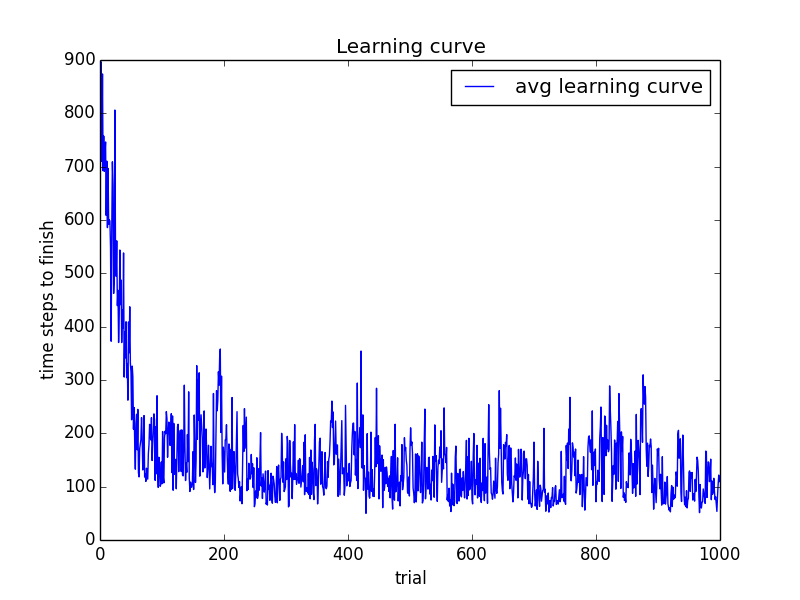
\includegraphics[width=0.8\textwidth]{figures/learning_curve.png}
\caption{Learning curve, averaged over $10$ independent learning agents.\label{fig:lcurve}}
\end{figure}

The learning curve of the implemented algorithm can be seen in the
Figure \ref{fig:lcurve}. It is an average over $10$ independent learning runs in
order to reduce the high oscillations of a single run. The initial drop in the curve
shows how the agent takes less time to 
complete the track. In Fig. \ref{fig:lcurve} the latency decreases from 900 to around 130 time steps on average before the 50th trial. In other words, the agent indeed learns the topology of the track
and the location of the reward. The learning curve plateaus after
approximately $100$ trials and after that the latency stops decreasing and
oscillates instead, between the values of $100$ and $300$. This shows that the agent has learned enough information
about the environment and starts to exploit it extensively. The exploration that
happens ($\epsilon = 0.1$ or 10$\%$ of the time) is not enough to find the better solutions.

\paragraph{Integrated reward}

\begin{figure}[h!]
\centering
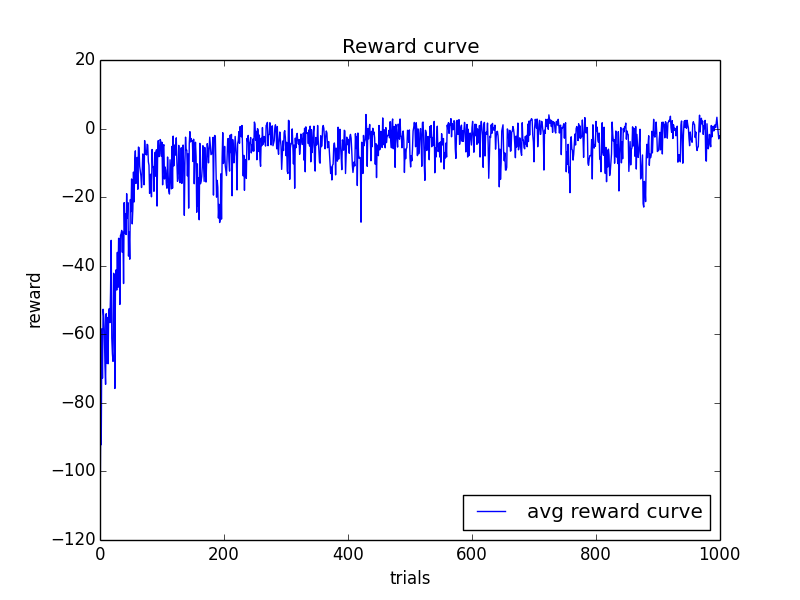
\includegraphics[width=0.8\textwidth]{figures/reward_curve.png}
\caption{Reward curve, averaged over 10 independent learning agents. \label{fig:rcurve}}
\end{figure}

The reward curve is plotted in the Figure \ref{fig:rcurve}. Qualitatively, it resembles
the learning curve, despite being negative and scaled. The consistency between
the two curves confirms the correlation between the reward obtained and the
learning.

\paragraph{Exploration-exploitation}



\paragraph{Navigation map}


\section{Car race}
comment on our changes (if we actually do this)
